
\section{Die Bewegung des Doppelpendels}
\subsection{Was ist ein chaotisches System?}
Typische Eigenschaften von chaotischen Systemen sind, dass sie mindestens drei Freiheitsgrade besitzen, ihre zugehörigen Differentialgleichungen nicht linear sind und dass es labile Zustände gibt. \citep{wikichaos}
Ein Doppelpendel hat auf den ersten Blick vier Freiheitsgrade: zwei Winkel und zwei Impulse.
Falls man allerdings Reibung und ähnliches außen vor lässt, gilt in dem abgeschlossenen System der Energieerhaltungssatz, sodass ein Freiheitsgrad verschwindet.
Ein typischer labiler Zustand liegt zum Beispiel vor, wenn das Pendel mit einem sehr geringen Impuls fast senkrecht nach oben zeigt.
Hier hängt der weitere Verlauf stark von kleinen Unterschieden in Position und Impuls ab.

Auf dieses Phänomen wird oft mit dem Ausdruck "`Schmetterlingseffekt"' Bezug genommen.
Interessant ist, dass die Systeme eigentlich deterministisch sind und mithilfe der Startbedingungen aus den Newton'schen Gleichungen der weitere Verlauf vollständig berechnet werden könnte.
Messfehler und Ungenauigkeiten in der Berechnung führen allerdings zu Fehlern, die sich in labilen Zuständen so stark auswirken, dass eine Simulation nach sehr kurzer Zeit erheblich von der Realität abweicht.

\subsection{Euler-Lagrange-Gleichung}
Der Lösungsansatz über die Euler"=Lagrange"=Gleichung ist von der englischen Wikipedia übernommen worden.
\citep{wikidoublependulum}

Die Gleichungen wurden allerdings um die Konstanten $k_1$ bis $k_5$ erweitert, um sie an unser Pendel anpassen zu können, das keine gleichmäßige Massenverteilung aufweist.

Die Positionen der Pendelarme können durch die zwei generalisierten Koordinaten $\phi_1$ und $\phi_2$ beschrieben werden, welche die Winkel der Arme angeben.
Alle Winkel werden relativ zur Ruhelage angegeben, also bedeutet $0^\circ$, dass ein Pendelarm senkrecht nach unten zeigt, während er bei $45^\circ$ nach unten rechts zeigt.
Für die vollständige Angabe des Zustands des Systems ist zusätzlich noch der generalisierte Impuls, hier als $p_1$ und $p_2$ bezeichnet, vonnöten.

Aus dem System von Differentialgleichungen für $p_1$, $p_2$, $\phi_1$ und $\phi_2$ lässt sich aus dem aktuellen Zustand der Zustand des Systems zu jeder gegebenen Zeit berechnen.
Die Berechnung kann zum Beispiel iterativ mit dem Runge"=Kutta"=Verfahren vierter Ordnung erfolgen.
\citep{wikirungekutta}

\begin{figure}[bht]
  \includegraphics[width=\textwidth]{charts/mathsketch_dia.png}
  \caption{Zeichnung der Pendelarme zur Bedeutung der Längenangaben}
  \label{fig:mathsketch}
\end{figure}

In Abbildung \ref{fig:mathsketch} ist dargestellt, wie die Längenangaben zu interpretieren sind.
An der ersten Achse ist das Doppelpendel aufgehängt.
$l_{1a}$ ist eine negative Zahl und gibt an, wie lang das erste Pendel auf der Seite ist, an der nicht das zweite Pendel hängt.
$l_1$ gibt den Abstand der beiden Achsen an und $l_{1b}$ beschreibt als positive Zahl die Länge des ersten Pendels in Richtung des zweiten Pendels.
$l_{2a}$ und $l_{2b}$ geben die beiden Längen des zweiten Pendelarms relativ zu seiner Achse an.

Diese Längenangaben sind in den Konstanten $k_1$ bis $k_5$ wiederzufinden, die darauf abzielen, die Eigenschaften des Pendels so genau wie möglich beschreiben zu können, indem zwei Dichtefunktionen $\rho_1(r)$ und $\rho_2(r)$ für die Massenverteilung über den Abstand $r$ von der jeweiligen Achse für die beiden Pendelarme angegeben werden:

\mathematik
k_1 &= \int^{l_{1b}}_{l_{1a}} \rho_1(r) \; r^2 \intend r
\qquad && k_2 &= \int^{l_{1b}}_{l_{1a}} \rho_1(r) \; r \intend r \\
k_3 &= \int^{l_{2b}}_{l_{2a}} \rho_2(r) \intend r
&& k_4 &= \int^{l_{2b}}_{l_{2a}} \rho_2(r) \; r^2 \intend r \\
k_5 &= \int^{l_{2b}}_{l_{2a}} \rho_2(r) \; r \intend r \\
\mathematikstop

Die folgenden Formeln beschreiben die Energien, die später auch in der Simulation gezeigt werden, und die durch die Konstanten $k_1$ bis $k_5$ bestimmt sind. Diese Konstanten entstehen aus einer Integration über die Massenverteilung; beispielsweise wird $T_1 = \int^{l_{1b}}_{l_{1a}} \half \rho_1(r) (r \cdot \phid_1)^2 \intend r$, wo $\half \rho_1(r) (r \phid_1)^2$ die kinetische Energie eines Massenelements angibt, zu:

\mathematik
T_1 &= \half k_1 \phid_1^2 & V_1 &= -g k_2 cos \phi_1 \\
T_2 &= \half l_1^2 k_3 \phid_1^2 + \half k_4 \phid_2^2 + l_1 \phid_1 \phid_2 k_5 cos(\phi_1 - \phi_2) & V_2 &= -g l_1 k_3 cos \phi_1 - g k_5 cos \phi_2 \\
\mathematikstop

Die Gesamtenergie im System beträgt $E = T_1 + T_2 + V_1 + V_2$.

Die Lagrange-Funktion $L$ ist dann:

\mathematik
L &= && T_1 + T_2 - (V_1 + V_2) \\
  &= && \half  \phid_1^2 k_1 + \half l_1^2 \phid_1^2 k_3 + \half \phid_2^2 k_4 + l_1 \phid_1 \phid_2 k_5 cos(\phi_1 - \phi_2) \\
  &&& + g k_2  cos \phi_1 + g l_1 k_3 cos \phi_1 + g k_5 cos \phi_2
\mathematikstop

Daraus ergeben sich folgende Euler-Lagrange-Gleichungen:

\mathematik
\dot{p}_1 - \frac{\partial L}{\partial \phi_1} &= 0 \qquad &\text{mit}\quad && p_1 = \frac{\partial L}{\partial \phid_1} \\
\dot{p}_2 - \frac{\partial L}{\partial \phi_2} &= 0        &\text{mit}\quad && p_2 = \frac{\partial L}{\partial \phid_2}\\
\mathematikstop

Nach Auflösung zu den Ableitungen lauten die Differentialgleichungen wie folgt:

\mathematik
\phid_1 &= \frac{k_4 p_1 - k_5 l_1 p_2 cos(\phi_1 - \phi_2)}{k_1 k_4 + l_1^2 \cdot (k_3 k_4 - k_5^2 cos^2(\phi_1 - \phi_2))} \\[0.5\baselineskip]
\phid_2 &= \frac{k_1 p_2 + l_1 \cdot (k_3 l_1 p_2 - k_5 p_1 cos(\phi_1 - \phi_2))}{k_1 k_4 + l_1^2 \cdot (k_3 k_4 - k_5^2 cos^2(\phi_1 - \phi_2))} \\[0.5\baselineskip]
\dot{p}_1 &= -l_1 \phid_1 \phid_2 k_5 sin(\phi_1 - \phi_2) - g k_2 sin \phi_1 - g l_1 k_3 sin \phi_1 \\[0.5\baselineskip]
\dot{p}_2 &= l_1 \phid_1 \phid_2 k_5 sin(\phi_1 - \phi_2) - g k_5 sin \phi_2 \\[0.5\baselineskip]
\mathematikstop

Nun werden auf der rechten Seite der Gleichungen für $\dot{p}_1$ und $\dot{p}_2$ noch $\phid_1$ und $\phid_2$ durch die rechte Seite der ersten zwei Gleichungen ersetzt, um eine Standardform für die Berechnung mithilfe des Runge"=Kutta"=Verfahrens zu erreichen.

\subsection{Linearisierung der Bewegungsgleichungen}
%TODO linearisierung
%TODO theoretische bestimmung der eigenfrequenzen

\subsection{Numerische Simulation mit Haskell/C}

Wir haben in Haskell eine Simulation geschrieben, die das klassische Runge"=Kutta"=Verfahren anwendet, da sich diese Sprache gut für Mathematik und den Umgang mit Formeln eignet. Die funktionierende Haskell-Implementierung haben wir dann aus Geschwindigkeitsgründen nach C portiert.

Die Simulation generiert eine CSV-Datei, in die in regelmäßigen Zeitintervallen die Winkel und die verschiedenen Energien geschrieben werden.
Auf die Winkel wird danach die diskrete Fourier"=Transformation mit einem sich bewegenden Fenster angewendet, um Perioden in der Bewegung erkennen zu können.
Nachdem die Winkel und ihre Transformationen berechnet sind, werden die Daten angezeigt.
In Abbildung \ref{fig:hssim} ist ein Screenshot der Anzeige zu sehen.

\begin{figure}[bht]
  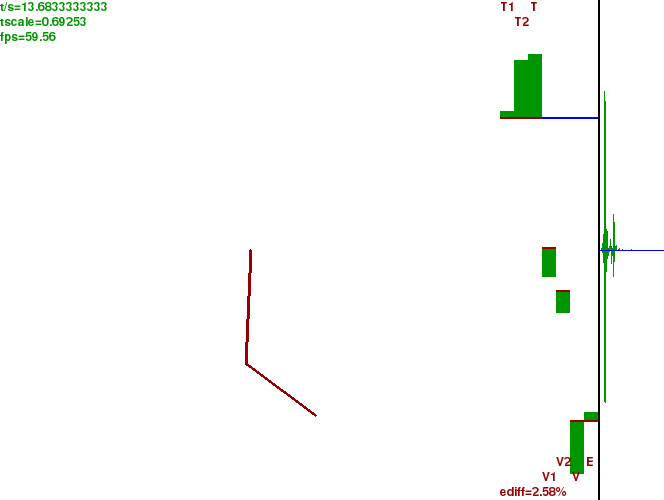
\includegraphics[width=\textwidth]{images/haskell_simulation_fwindow1000_whitebg_cropped.png}
  \caption{Screenshot der Simulation}
  \label{fig:hssim}
\end{figure}

Zu erkennen ist die aktuelle Position des Pendels als rote Skizze der Arme.
Die dicken grünen Balken rechts daneben zeigen auf einer für alle dicken Balken gleichen Skalierung die Energien $T_1$, $T_2$, $T_{Ges}$, $V_1$, $V_2$, $V_{Ges}$ und $E_{Ges}$ in der Reihenfolge von links nach rechts an.
Der blaue Stricht zeigt die Nulllinie an, die roten Striche die Anfangswerte der Energien.
Die potentielle Energie ist anfangs kleiner als null, weil der Koordinatenurspung in der ersten Achse liegt und damit die Schwerpunkte der Pendelarme unterhalb des Bezugspunkts liegen.
Die Gesamtenergie $E_{Ges}$ sollte bei einer perfekten Simulation nicht von ihrem Anfangswert abweichen, aber wie zu sehen ist, wächst sie in unserer Simulation stetig.
Dies ist auf die Ungenauigkeiten der numerischen Simulation zurückzuführen.

Rechts neben den dicken Balken ist die diskrete Fourier"=Transformation der Winkel zu sehen.
Oberhalb der blauen Linie wird die Transformation von $\phi_1$ angezeigt, unterhalb die Transformation von $\phi_2$.
Jeder der Balken ist einen Pixel breit und bedeutet eine Frequenz aus dem Ergebnis.
Der Abstand nach rechts vom ersten Balken aus ist proportional zur Frequenz.
Aus dem aktuell zu sehenden Fester ist zum Beispiel für den ersten Pendelarm abzulesen, dass sich das Pendel regelmäßg von rechts nach links bewegt, zu erkennen am rechten Ausschlag, und der zweite Pendelarm eine schwächere aber schnellere Schwingung erzeugt, zu sehen als linker Ausschlag.

Die Transformation des zweiten Pendelarms zeigt eine starke Korrelation mit der Transformation des ersten Pendelarms. Das liegt daran, dass für diese Abbildung eine relativ stark periodische Einstellung des Systems gewählt wurde und der zweite Pendelarm eine dem ersten Pendelarm ähnliche Bewegung durchführt.

\subsection{Untersuchung des Frequenzspektrums}

\begin{figure}[bht]
  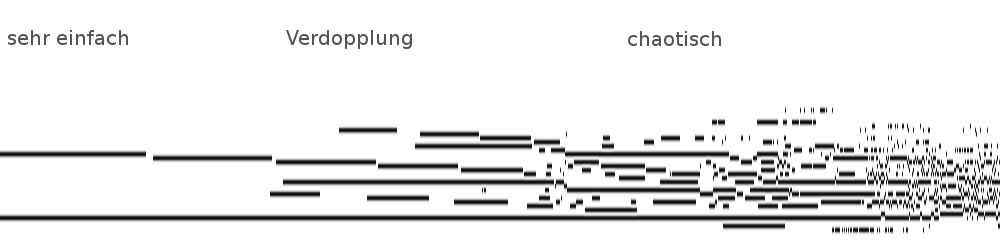
\includegraphics[width=\textwidth]{images/frequencies_text.png}
  \caption{Frequenzanalysen bei verschiedenen Starbedingungen.}
  \label{fig:frequencies}
\end{figure}

Wenn die Simulation sehr oft durchgeführt wird und bei jeder Ausführung der Startwinkel $\phi_1$ um einen kleinen Schritt vergrößert wird, kann das Verhalten des Systems bei verschiedenen Energien untersucht werden.
Der Winkel des zweiten Pendelarms wird dabei immer mit der doppelten Größe initialisiert: $\phi_2 = 2\phi_1$.

In Abbildung \ref{fig:frequencies} ist ein Diagramm zu sehen, in dem von links nach rechts die Startbedingungen mit $\phi_1$ linear von $0\;rad$ bis $\pi/4\;rad$ vergrößert werden.
Auf der vertikalen Achse sind die Positionen der Maxima aus der Fourieranalyse für die ersten 12 Sekunden der Simulation aufgetragen. Je höher dort ein schwarzer Punkt liegt, desto höher ist die Frequenz.

Auf den ersten Blick sind mehrere Abschnitte zu sehen, in denen das Pendel in verschieden vielen Frequenzen schwingt: Im ersten Bereich sind nur zwei Frequenzen vorhanden. Danach ist eine Verdopplung der Frequenzen zu beobachten und dann der Übergang in den chaotischen Bereich, in dem sehr viele Frequenzen zu finden sind. Am rechten Rand des Diagramms ist schön zu erkennen, wie sehr kleine Änderungen in den Startbedingungen bei großen Energien so starke Abweichungen hervorrufen, dass sie sich sofort im Diagramm niederschlagen.

Interessant ist, dass es eine Grundschwingung gibt, die die ganze Zeit gleich bleibt, und sich erst im allerletzten Teil ein wenig verändert.
Diese Grundschwingung ist auf die konstante Massenverteilung zurückzuführen, die eine bestimmte Periode bestimmt, ähnlich eines einfachen Pendels.

\subsection{Untersuchung des Phasenraums}

%TODO bilder, text, ...


\subsection{Überschlagsdiagramm \TODO}

%TODO jann?

